\documentclass[10pt]{article}
\usepackage[T1]{fontenc}
\usepackage[margin=0.62in]{geometry}
\usepackage{array}
\usepackage{tikz}
\usetikzlibrary{arrows.meta,positioning,calc}

\pagestyle{plain}
\setlength{\parindent}{0pt}
\setlength{\parskip}{0.28em}
\emergencystretch=3em
\renewcommand{\arraystretch}{1.08}

\newcolumntype{L}[1]{>{\raggedright\arraybackslash}p{#1}}
\tikzset{
  box/.style={draw, rounded corners=1pt, align=center, inner sep=4pt, minimum height=8mm},
  smallbox/.style={draw, rounded corners=1pt, align=center, inner sep=3pt, font=\scriptsize},
  edge/.style={-{Stealth[length=2mm]}, thick},
  faintedge/.style={-{Stealth[length=2mm]}, thick, dashed}
}

\begin{document}

\begin{center}
{\Large OpenFNIRS / OpenNIRScap}\\
{\normalsize Dense fNIRS build-state, board-flow, and fixed-board model}\\
worlds session, 2026-06-02
\end{center}

\section*{Verdict}

\begin{center}\small
\begin{tabular}{|L{1.05in}|L{4.35in}|L{0.65in}|}
\hline
\textbf{Plane} & \textbf{Dense status} & \textbf{Gate} \\
\hline
Identity & Open, non-invasive fNIRS acquisition stack: sensor modules, ECU,
ST-LINK adapter, cap/cables, STM32 firmware, Python host. & fixed \\
\hline
Local build & Eight sensor modules, one ECU, five ST-LINK adapter boards. Build is
at inspection and placement, not human-use readiness. & partial \\
\hline
Open blockers & Five of eight sensor J1 connectors stocked; ECU SW1 fit unknown;
TMUX population unknown; ST-LINK adapter headers incomplete. & hold \\
\hline
Success claim & Eight channels must pass connector, analog, power, mux, firmware,
USB frame, host MBLL/CBSI, cap-fit, optical, and isolation proofs. & proof \\
\hline
\end{tabular}
\end{center}

\section{Whole-stack fNIRS flow}

\begin{center}
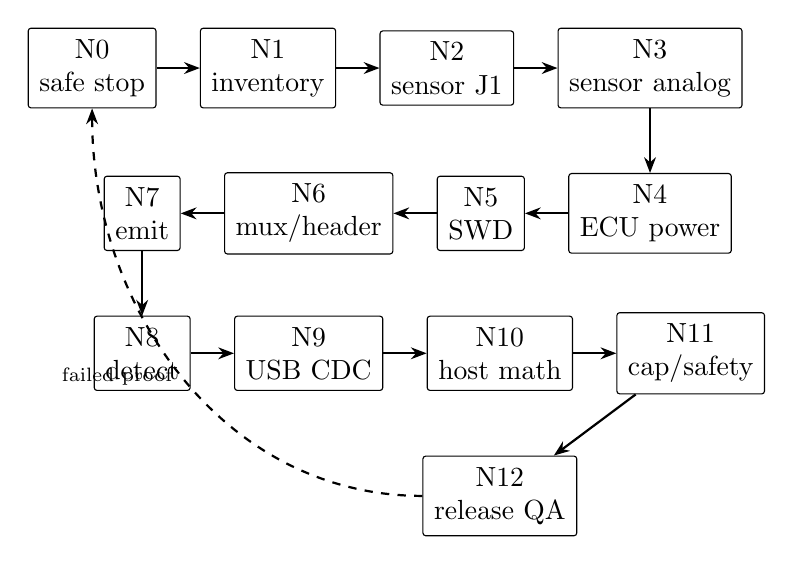
\begin{tikzpicture}[node distance=0.82cm and 0.55cm]
\node[box] (n0) {N0\\safe stop};
\node[box, right=of n0] (n1) {N1\\inventory};
\node[box, right=of n1] (n2) {N2\\sensor J1};
\node[box, right=of n2] (n3) {N3\\sensor analog};
\node[box, below=of n3] (n4) {N4\\ECU power};
\node[box, left=of n4] (n5) {N5\\SWD};
\node[box, left=of n5] (n6) {N6\\mux/header};
\node[box, left=of n6] (n7) {N7\\emit};
\node[box, below=of n7] (n8) {N8\\detect};
\node[box, right=of n8] (n9) {N9\\USB CDC};
\node[box, right=of n9] (n10) {N10\\host math};
\node[box, right=of n10] (n11) {N11\\cap/safety};
\node[box, below=of n10] (n12) {N12\\release QA};

\draw[edge] (n0) -- (n1);
\draw[edge] (n1) -- (n2);
\draw[edge] (n2) -- (n3);
\draw[edge] (n3) -- (n4);
\draw[edge] (n4) -- (n5);
\draw[edge] (n5) -- (n6);
\draw[edge] (n6) -- (n7);
\draw[edge] (n7) -- (n8);
\draw[edge] (n8) -- (n9);
\draw[edge] (n9) -- (n10);
\draw[edge] (n10) -- (n11);
\draw[edge] (n11) -- (n12);
\draw[faintedge] (n12.west) to[out=180,in=270] node[left, font=\scriptsize]{failed proof} (n0.south);
\end{tikzpicture}
\end{center}

\section{Actual board-state matrix}

\begin{center}\scriptsize
\begin{tabular}{|L{0.36in}|L{0.95in}|L{1.75in}|L{1.55in}|L{1.35in}|}
\hline
\textbf{S} & \textbf{Where} & \textbf{What / how} & \textbf{Why} & \textbf{Exit proof} \\
\hline
N0 & whole stack & LEDs off; USB disconnected unless bench-powered; no human subject. & Prevent software progress from implying safety. & Bench-only state. \\
\hline
N1 & inventory & Count eight sensor boards, one ECU, five adapters, headers, muxes, USB, regulator, switch. & Missing parts are state, not footnotes. & Population map. \\
\hline
N2 & sensor J1 & Populate/defer bottom-edge six-pad T1M-06-F-SH-L-K; stock covers five boards. & J1 is optode-to-ECU boundary. & Eight known orientations. \\
\hline
N3 & sensor analog & Verify/place C3 200 pF C0G; probe R1 60.4 k and R2 3.9 M before hand-add. & LED/PD/TIA creates voltage from light. & Dark/light response. \\
\hline
N4 & ECU power/USB & Fit U3 LM1085, J2 Mini-B, SW1 only after footprint check; prove rail first. & ECU owns power and transport. & 3.3 V, reset, USB. \\
\hline
N5 & ECU SWD/adapter & ECU J3 uses reserved FTSH; adapter needs HTSW J1 and second FTSH J2. & Flash path must be repeatable. & Fresh flash, no improvised wires. \\
\hline
N6 & ECU mux/headers & Place eight T1M-10 headers; inspect TMUX1104 positions; map select lines to channel order. & Mux defines which sensor reaches ADC. & Truth table plus ADC response. \\
\hline
N7 & emitter & STM32 timers/GPIO expander sequence 660/940 nm LEDs on selected module. & fNIRS depends on wavelength and timing. & LED current/optical bound. \\
\hline
N8 & detector & Photodiode/TIA returns analog signal through connector to ECU ADC DMA. & This is the hardware data point. & Non-saturated samples. \\
\hline
N9 & USB CDC & Frame channel, wavelength, timing, ADC values to host. & Host cannot recover lost provenance. & Serial frame log. \\
\hline
N10 & host & Python ingest, live traces, MBLL, CBSI, plots, CSV. & Converts board data to fNIRS features. & Controlled test plots/files. \\
\hline
N11 & cap/safety & Cable mates, strain relief, optode spacing, skin contact, shielding, isolation. & Bench-safe is not body-safe. & Safety checklist. \\
\hline
N12 & release & Save photos, BOM, firmware hash, channel map, rail/optical/USB/host evidence. & Reproducibility gate. & Full evidence bundle. \\
\hline
\end{tabular}
\end{center}

\section{Counterfactual fixed board stack}

\begin{center}
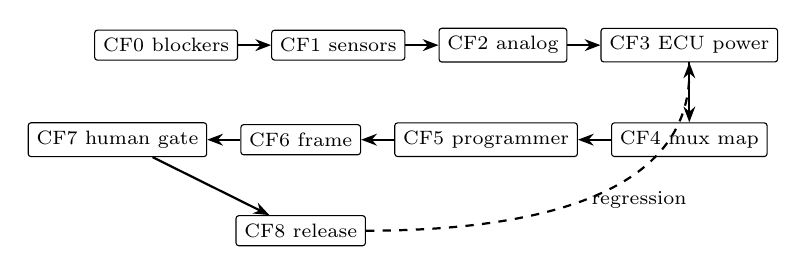
\begin{tikzpicture}[node distance=0.76cm and 0.42cm]
\node[smallbox] (c0) {CF0 blockers};
\node[smallbox, right=of c0] (c1) {CF1 sensors};
\node[smallbox, right=of c1] (c2) {CF2 analog};
\node[smallbox, right=of c2] (c3) {CF3 ECU power};
\node[smallbox, below=of c3] (c4) {CF4 mux map};
\node[smallbox, left=of c4] (c5) {CF5 programmer};
\node[smallbox, left=of c5] (c6) {CF6 frame};
\node[smallbox, left=of c6] (c7) {CF7 human gate};
\node[smallbox, below=of c6] (c8) {CF8 release};
\draw[edge] (c0) -- (c1);
\draw[edge] (c1) -- (c2);
\draw[edge] (c2) -- (c3);
\draw[edge] (c3) -- (c4);
\draw[edge] (c4) -- (c5);
\draw[edge] (c5) -- (c6);
\draw[edge] (c6) -- (c7);
\draw[edge] (c7) -- (c8);
\draw[faintedge] (c8.east) to[out=0,in=270] node[right, font=\scriptsize]{regression} (c3.south);
\end{tikzpicture}
\end{center}

\begin{center}\scriptsize
\begin{tabular}{|L{0.42in}|L{1.0in}|L{2.55in}|L{1.85in}|}
\hline
\textbf{CF} & \textbf{Fix plane} & \textbf{Counterfactual board/stack change} & \textbf{Dense criterion} \\
\hline
CF0 & current blockers & Name incomplete connector count, unknown SW1 fit, unknown mux population, missing adapter headers. & No final claim while blockers exist. \\
\hline
CF1 & sensors & All eight J1 connectors populated, oriented, and mapped to cable-side mates. & No silent channel exclusion. \\
\hline
CF2 & analog & C3/R1/R2 decisions locked; LED/photodiode/TIA behavior measured per module. & Eight dark/active traces. \\
\hline
CF3 & ECU power & U3/J2/SW1 footprint-correct; test pads and rail gates explicit. & Rail, reset, USB logs. \\
\hline
CF4 & mux/channel & T1M-10 headers and TMUX positions known; firmware channel order matches BOM/silkscreen. & Mux truth table. \\
\hline
CF5 & programming & Adapter headers complete or equivalent cable documented. & Flash from reset ECU. \\
\hline
CF6 & frame contract & USB frame names channel, wavelength, sample timing, ADC scale, cap position. & Firmware labels match plots/CSV. \\
\hline
CF7 & human-use gate & Optical power, isolation, strain relief, shielding, contact procedure explicit. & Signed bench safety gate. \\
\hline
CF8 & released stack & Eight channels stream through ECU, USB, MBLL/CBSI, and saved controlled-test artifacts. & Dataset, plots, photos, hashes. \\
\hline
\end{tabular}
\end{center}

\section{Disentangled fNIRS+EEG exoprior model}

\begin{center}\scriptsize
\begin{tabular}{|L{0.9in}|L{1.45in}|L{1.45in}|L{2.2in}|}
\hline
\textbf{Latent} & \textbf{EEG projection} & \textbf{fNIRS projection} & \textbf{Counterfactual split} \\
\hline
Intent & ERP, SSVEP, MI, phase, band shifts at sub-second scale. & Not a direct controller; delayed hemodynamic correlate at best. & If EEG is delayed/shuffled, fast action confidence should collapse. \\
\hline
Capacity & Alpha/beta/gamma attention markers, artifact-sensitive. & HbO/HbR workload, fatigue, prefrontal engagement over seconds. & If fNIRS is delayed/shuffled, pacing and trust priors should degrade, not controls. \\
\hline
Context & Event-locked response to task, stimulus, error, and feedback. & Slow regime: visualization, memory load, overload, recovery. & Same player across tasks must separate trait from task mode. \\
\hline
Group state & Cross-player phase/attention synchrony where valid. & Cross-player workload readiness and recovery synchrony. & Swapped players test identity leakage; hidden social state tests metadata leakage. \\
\hline
Artifact & Motion, electrode contact, blink/muscle, line noise. & Motion, optode contact, hair/skin, ambient light, baseline drift. & Injected artifacts must route to artifact state, not cognition. \\
\hline
\end{tabular}
\end{center}

\begin{center}\scriptsize
\begin{tabular}{|L{1.15in}|L{2.15in}|L{2.75in}|}
\hline
\textbf{Model plane} & \textbf{Dense rule} & \textbf{Released exoprior token} \\
\hline
Fast action & Fit \(P(action \mid EEG, world)\); do not early-fuse raw optical data. & Intent confidence, selected action, timing confidence. \\
\hline
Slow capacity & Fit \(P(capacity \mid fNIRS, behavior, world)\); respect hemodynamic lag. & Workload, fatigue trend, readiness, recovery state. \\
\hline
World state & Condition on task, turn, error, stimulus, latency, and social role. & Role, phase, objective pressure, recent outcome. \\
\hline
Fusion & Late-fuse derived latents, not raw EEG/fNIRS. & Player state: \{intent, capacity, context, trust, artifact\}. \\
\hline
Multiplayer policy & Adapt pacing, turn timing, trust weighting, difficulty, and feedback. & Group state without exposing raw neural traces. \\
\hline
\end{tabular}
\end{center}

\textbf{Disentangling claim.} EEG supplies fast intentional evidence; fNIRS supplies
slow capacity/context evidence. The multiplayer layer may consume only derived
exopriors, never raw neural streams, and each claim must survive the corresponding
shuffle, delay, swapped-player, hidden-metadata, and artifact-injection
counterfactual.

\section{BOM and build gates}

\begin{center}\scriptsize
\begin{tabular}{|L{1.15in}|L{1.55in}|L{3.15in}|}
\hline
\textbf{Area} & \textbf{Stock / evidence} & \textbf{Action gate} \\
\hline
Sensor boards & 8 boards; T1M-06 x5; C3/R1/R2 stock & Need 8 J1 total; verify C3/R1/R2 before hand-add. \\
\hline
ECU power/USB & LM1085 x2; Mini-B x2; tactile x3 & Fit-check SW1; prove U3 rail and J2 enumeration. \\
\hline
ECU mux/bus & T1M-10 x8; TMUX1104 x8; FTSH x1 & Inspect mux population; populate headers; map channel order. \\
\hline
ST-LINK adapter & 5 bare boards; missing HTSW; extra FTSH needed & Buy/populate adapter headers before treating flash path as ready. \\
\hline
Set aside & AD8618ARUZ, 1N5819W, S1SS mates, unmatched E4F & Do not place without exact footprint/designator match. \\
\hline
Host software & upstream STM32 and Python paths & Frame contract must match channel/wavelength/cap map. \\
\hline
\end{tabular}
\end{center}

\section{Proof checklist}

\begin{center}\scriptsize
\begin{tabular}{|L{1.25in}|L{2.2in}|L{2.25in}|}
\hline
\textbf{Claim} & \textbf{Evidence required} & \textbf{Rollback if missing} \\
\hline
Board stack complete & Eight sensor photos, ECU photo, adapter photo, BOM counts. & Return to N1/N2/N5. \\
\hline
Electrical acquisition & 3.3 V rail, reset, mux truth table, ADC dark/light samples. & Return to N4/N6/N8. \\
\hline
Optical fNIRS timing & 660/940 current and optical bounds plus frame timing. & Return to N7/N9. \\
\hline
Host validity & USB frame log, Python plots, CSV, labels matching cap map. & Return to N9/N10. \\
\hline
Human-readiness & Optical power, isolation, strain relief, skin/contact, ambient shielding. & Remain bench-only N0/N11. \\
\hline
\end{tabular}
\end{center}

\section{Evidence and artifacts}

\begin{itemize}
\item \texttt{p/place/bci/devices/openfnirs-build.tree}: transcludable dense model.
\item \texttt{p/place/bci/stages/forester-bci-factory.tree}: BCI factory link.
\item \texttt{p/place/trees/bcf-0036.tree}: purchase/manufacturing/browser evidence.
\item \texttt{p/place/assets/gerbers/opennirscap-v2/}: ECU, sensor, ST-LINK gerbers.
\item \texttt{p/place/build/latex/openfnirs/openfnirs-state-machine.pdf}: this rendered artifact.
\item Upstream \texttt{tonykim07/fNIRS}: STM32 firmware and Python host.
\end{itemize}

\textbf{Safety.} Non-invasive fNIRS build-state artifact only. No clinical or
human-subject readiness is claimed until optical power, electrical isolation,
cabling, fit, and data-quality proofs pass.

\end{document}
